The function of this chapter is to get a deeper understanding of the modules and code that has been written. Due to time constraints and hardware failure, the following modules were not realized: "Lamp, Social, Wi-Fi, Controller, ADC, EEPROM". Thus these modules will not be discussed in this chapter. 
\subsection{platform}
We start with the most tightly with the microcontroller integrated layer.
\subsubsection{UART}
The UART module delivers all the communication to the USB-Serial converter and ESP8266. The code has been kept as generic as possible so that adjustments to the external hardware has no influence to the driver code. It would even be possible to move to a different xmega model with more USART ports since a macro is used for generating the interrupt code. Every USART port has a status, an array with delimiters, an in and output buffer, a sending status and an id. The status contains variables for the buffers, and allows for a ring-buffer usage. A ringbuffer is chosen as it has little overhead compared to lists or queues, the order of the data matters, and we don't expect to go outside of our given buffer capacity. The delimiters are used for the USART to listen to certain characters on the receiving data. Once there is a match an event will be fired. The example below shows the usage of this delimiter.
\begin{minted}[baselinestretch=1, fontsize=\small, linenos,frame=single,framesep=5pt]{C}
uint8_t uart_add_delimiter(char delimiter, USART_t * port);
static void callback(Event * event, uint8_t * data) {
	if(event == EVENT_UART_DELIMITER){
	struct UartDelimiter * delimiter = (struct UartDelimiter*)data;
		if (delimiter->port == &ESP_UART_PORT) {
			//Read buffers etc
		}
	}
}
static uint8_t init(void) {
	uart_add_delimiter('\n', &ESP_UART_PORT);
	event_addListener(&EVENT_UART_DELIMITER, callback);
	return 1;
}
\end{minted}
In this example, a certain module will tell the UART module to listen for a new line character, and the module will subscribe to the event. The UART module passes the delimiter information with it, so that there is knowledge about how much data can be read since the last delimiter event.\\ 
The interrupts are generated with the macros that can be found at appendix \ref{append:usartinterruptgen}.
The following following code can be used to generate the interrupt code for every USART channel:
\begin{minted}[baselinestretch=1, fontsize=\small, linenos,frame=single,framesep=5pt]{C}
USARTRXCISR(USARTE0, DEBUG_UART,     USARTE_ID, received);
USARTDREISR(USARTE0, DEBUG_UART,     USARTE_ID);
USARTRXCISR(USARTD1, ESP_UART_PORT,  USARTD_ID, );
USARTDREISR(USARTD1, ESP_UART_PORT,  USARTD_ID);
\end{minted}
Since the system could be writing to the buffer that is being handled in the interrupt, a lock has been implemented to prevent unexpected outcome. One lock waits while the lock signal is freed, while the other lock function returns a 0 upon failure to acquire the lock
\begin{minted}[baselinestretch=1, fontsize=\small, linenos,frame=single,framesep=5pt]{C}
#define lock(id) while (outBufferLock[id]); outBufferLock[id] = 1
#define unlock(id) outBufferLock[id] = 0

static inline uint8_t softlock(uint8_t id) {
	if (outBufferLock[id]) return 0;
	outBufferLock[id] = 1;
	return 1;
}
\end{minted}
The USART on both channels have the same settings. 8 bit words, medium level interrupts and a baudrate of 115200. This baudrate can go higher once the whole system is tested with good results.
\subsubsection{SPI}
The SPI driver is incomplete as is, a lot of performance optimizations can and should be done. One of the biggest pitfalls at the moment is that it is blocked writing. When a lot of data is being sent consecutively by the SPI driver, the event buffer fills up and might even get full. Interrupt based design should be looked at and investigated, as this would still allow the events to be handled. The caveat with this, however, is that a large buffer has to be allocated for the SPI. And memory is costly. DMA is another technique to be looked at, this would eliminate the need for a CPU at all and give the system all the time to process the other tasks. There needs to be some caution, as DMA has overhead on low data. This should be investigated.
\subsubsection{Timer}
The Timer design is incomplete, and only houses a RTC. Due to a hardware failure, the internal crystal is being used. Which offers a worse accuracy than an external one. However since the most recent time can be retrieved from the internet this is not a major issue. Future additions to the Timer module include: Alarm function for timeouts on waiting, PWM functionality and using the 32 RTC with the external crystal. The Timer module is set up to use it's overflow interrupt. If the internal counter overflows the period of 1023 a second pulse event will get fired and the run time will get incremented.
\subsection{Driver}
One step up gives the communication with external hardware.
\subsubsection{SEPS525F}
As mentioned before, the screen uses a SEPS525F ic. This driver drives allows for driving screens with a resolution of up to 160x128 pixels with 18 bit combined color. This means that there are 6 bits for blue, 6 bits for green and 6 bits for red. However this would require to send 3 bytes for 2 bits of color precision. There is also a 16 bits combined color option available, which has been used in this driver. 5 bits for blue, 6 bits for green and 5 bits for red. A 24 bit color (8 bits per color, 0-255) can be converted with the following define:
\begin{minted}[baselinestretch=1, fontsize=\small, linenos,frame=single,framesep=5pt]{C}
#define SEPS525F_TO656(r,g,b)((r>>3)<<11)|((g>>2)<<5)|(b>>3)
\end{minted}
The SEPS525F has three data interfaces that could be used: SPI, RGB, Parallel. In retrospect a parallel interface would've given major performance advantages. However due to time constraints a SPI interface has been chosen. The clock frequency of the SPI is set at the cpu speed divided by two. Which is a clock of 8 MHz when not in any power saving mode.\newpar
The SEPS525F has two modes, a data mode and a command mode. With the command mode a register can be set. In order to achieve this the register will be written first, while clearing the RS and the CS pin. Once the register is written, the RS pin will be set while keeping the CS pin low. After the data is written the CS pin will be set.
\begin{minted}[baselinestretch=1, fontsize=\small, linenos,frame=single,framesep=5pt]{C}
static void SEPS525F_reg(int idx, int value) {
	SEPS525F_PORT.OUTCLR = SEPS525F_CSB | SEPS525F_RS;
	spi_write_blocked(idx);
	SEPS525F_PORT.OUTSET = SEPS525F_RS;
	SEPS525F_PORT.OUTCLR = SEPS525F_CSB;
	spi_write_blocked(value);
	SEPS525F_PORT.OUTSET = SEPS525F_CSB;
}
\end{minted}
This can be seen in the code above. The driver gives the possibility to draw a single pixel, but it's significantly faster to write multiple pixels at once. For this a region that will be drawn on has to be set. Then the driver ic will expect a certain amount of pixels, which have to be written as data. According to the datasheet special scrolling features should be available, however this is not explained later on in the datasheet. There are a lot of parameters that can be set for the screen, such as duty cycle, frame rate, driving currents. The explanation of all these can be found in the datasheet, just like the recommended values. The given initialization sequence of the datasheet did not work, so an Arduino library has been ported successfully \textbf{Source}.
\subsubsection{Terminal}
The Terminal driver gives the possibility to format strings, and outputs the formatted strings to a sink. The default sink writes to the USB-Serial ic via the UART driver. Formatting is done via the tinyprint library \textbf{Source} and implements the "'d' 'u' 'c' 's' 'x' 'X'" formats.
\subsubsection{ESP8266}
The ESP8266 is a low cost Wi-Fi module which can be flashed with own firmware. In a next version this own firmware will be developed, however for now the standard firmware is used. UART is used to communicate with the module, via an Hayes command set based protocol\textbf{Source http://nemesis.lonestar.org/reference/telecom/modems/at/history.html}. The commands implemented allow for basic HTTP get requests. Due to time constraints it was not possible to finalize the usage of the module. Networks can be scanned, and a connection with a wireless action point can be established. But there is no functionality beyond that
\subsection{Modules}
Although all the drivers talked about before make use of the Module system, they are not taken place on the Module layer. This is a naming convention error.
\subsubsection{Command}
The Command module has the purpose of setting up an accessible possibility to execute commands received by the USB-Serial connection. It is possible to register up to 26 commands. One for every letter in the alphabet. A command can be registered by use of the following code:
\begin{minted}[baselinestretch=1, fontsize=\small, linenos,frame=single,framesep=5pt]{C}
command_hook_description(
	'T', &terminalCommand, "Log sink    T<option> options: U(Uart) S(Screen)\0"
);
\end{minted}
It takes 3 arguments, the first one being the letter the command is tied to. The second one is a function pointer for the callback. And the third one is a usage description that can be requested by the user by writing a '?' to the terminal. In fig. \ref{fig:command_usage} an example output can be seen.
\begin{figure}[H]
	\centering
	\label{fig:command_usage}
	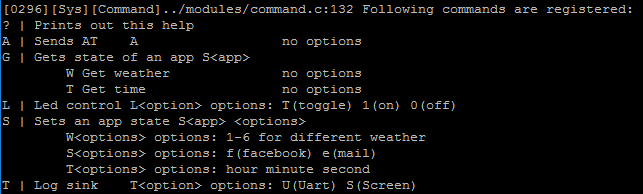
\includegraphics[width=1\textwidth]{./fig/command_usage.png}
	\caption{Response of a question mark}
\end{figure}
It's up to the developer to parse the string that is passed with the command. An example input string could be:"ST 12 23 34" which sets the time to 12:23:34. The callback will receive the same string as thats sent, minus the command character. Some helper functions have been written such as "command\_next\_int" to make parsing easier. Parsing the example string is done in the following code:
\begin{minted}[baselinestretch=1, fontsize=\small, linenos,frame=single,framesep=5pt]{C}
uint8_t index = 1;
if(data[index-1] == 'T'){
	uint32_t hour = command_next_int(&index, data, len);
	uint32_t minute = command_next_int(&index, data, len);
	uint32_t second = command_next_int(&index, data, len);
}
\end{minted}
\subsubsection{LOG}
Almost every driver or module has a dependency on the LOG driver. In order to use the logging functionality, a file first has to initialize the logger. this is done by calling:
\begin{minted}[baselinestretch=1, fontsize=\small, linenos,frame=single,framesep=5pt]{C}
LOG_INIT("Core");
\end{minted}
This is required to keep track of where the logging happens. There are multiple levels of logging, which currently all have the same effect other than the name, except for the "LOG\_ERROR" function. The error log function halts the system. In a future build there should be a possibility to set a general log level so that log statements with less importance than the general log level wont be written. Every log is translated to the following three statements:
\begin{minted}[baselinestretch=1, fontsize=\small, linenos,frame=single,framesep=5pt]{C}
#define LOG_INTERNAL(LEVEL, MSG, ...) \
	log_message("[%04d][%s][%s]%s:%d ",timer_runTime(),LEVEL,log_name,__FILE__,__LINE__);   \
	log_message_p(PSTR(MSG), ##__VA_ARGS__);                                                        \
	log_message("\r\n")
\end{minted}
An example like:
\begin{minted}[baselinestretch=1, fontsize=\small, linenos,frame=single,framesep=5pt]{C}
LOG_SYSTEM("Received command: %c", command);	//command is a character
\end{minted}
Produces the following string on the sink: "[2727][Sys][Command]../modules/command.c:157 Received command: T". The string contains the absolute runtime, what kind of log it was (debug, system, warning), the filename and the file line. The strings are saved in the flash to save memory. If the sink for the terminal changes, so does the output for the logger, as its depending on the terminal. The screen can be used to log to. This can be seen in fig. \ref{fig:screen_logger}.
\begin{figure}[H]
	\centering
	\label{fig:screen_logger}
	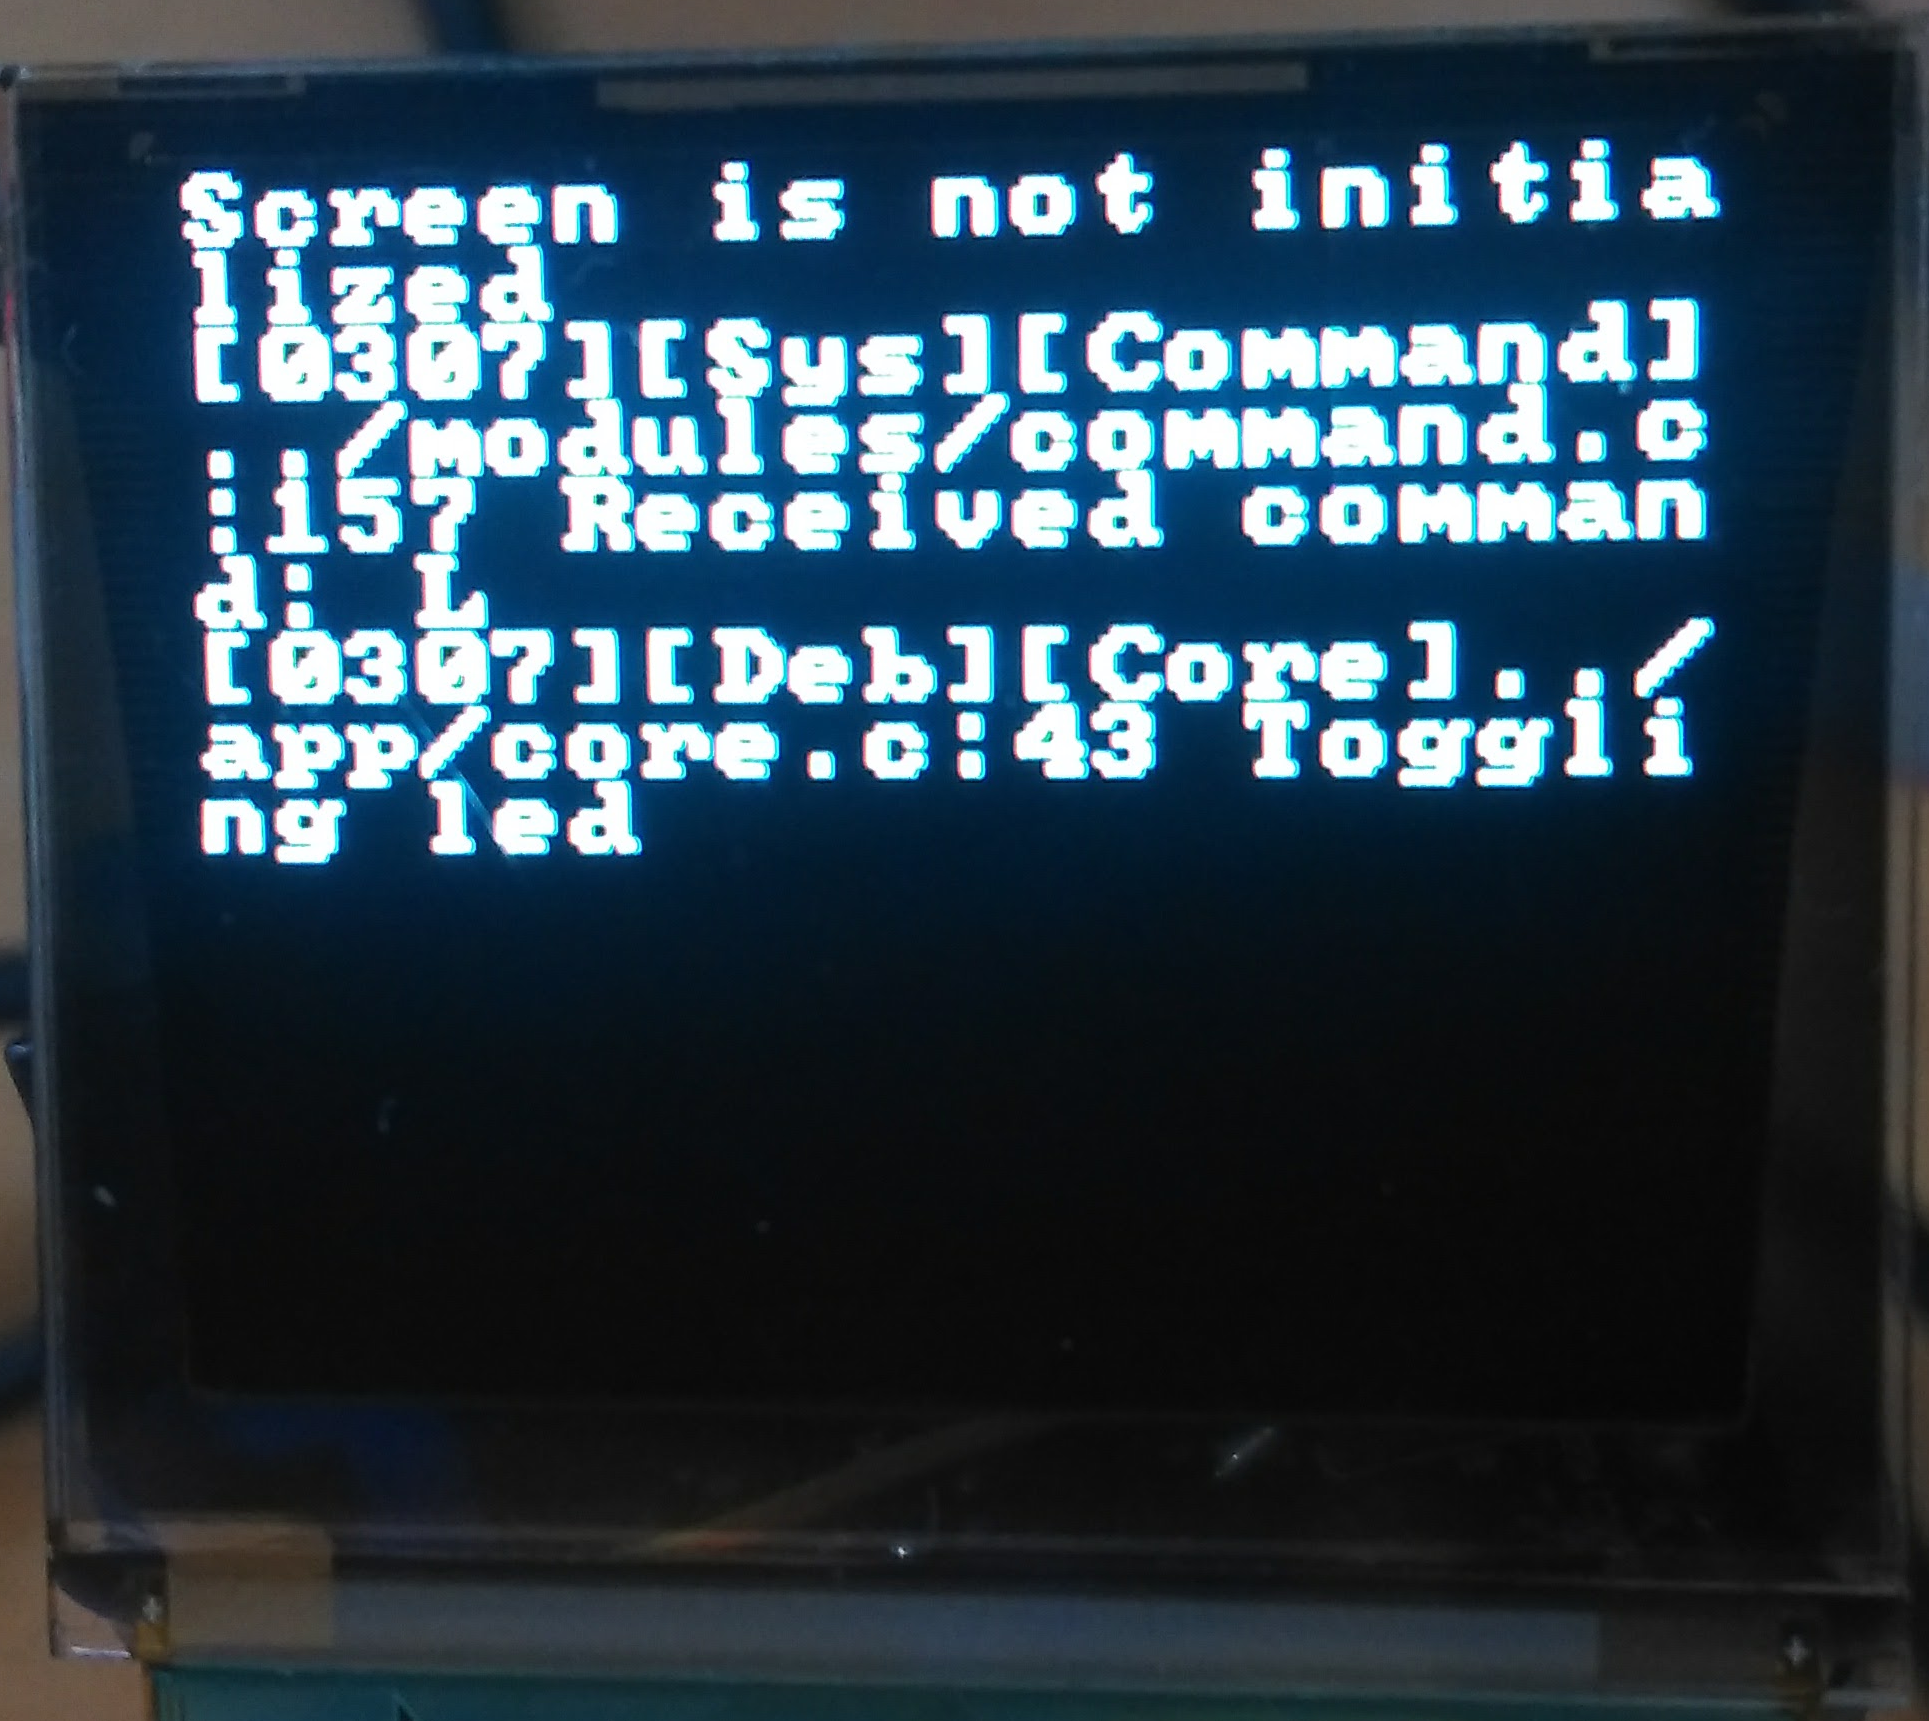
\includegraphics[width=0.4\textwidth]{./fig/screen_logger.png}
	\caption{Redirecting the output to the screen}
\end{figure}
However this has to be used carefully, as writing to screen takes significantly longer than outputting it over UART. So the system might freeze in case of too much text to show.
\subsubsection{Screen}
The Screen module contains routines for drawing shapes, images and text on the screen. Currently implemented shapes include: rectangle, filled rectangle, circle, filled circle, pixel, and line. These shapes are drawn with the color thats currently set. Images can be drawn both from flash and from memory. Better practice reads them out from flash, as there is little memory available. A start and stop function is available. This can be used to denote whether the shapes should be filled, or whether only the outline should be drawn. Another future addition can speed up the drawing significantly when a data start and data end command will be sent upon calling start and stop. This is not implemented in the current version.
\subsubsection{Time}
The Time keeps track of time offline. It does so by keeping track of hours minutes and seconds, and incrementing them accordingly upon every second pulse generated by the Timer driver. The time can also be set via a function.
\subsection{App}
This layer is the least elaborated, as it has the last priority since it wouldn't work without the layers before it regardless.
\subsubsection{clock}
The clock application draws a clock, analogue and digital. It gets update every second pulse, and also redraws in that case. The SPI connection is not capable enough to show a smooth analogue clock as is, which causes slight stutters when drawing. This behavior could be resolved when programming even more efficiently, one way of tackling this problem would be to draw the lines first to a buffer, which then is drawn as an image. This would provide a more efficient pipeline for drawing the clock, at the cost of memory. Otherwise a compromise will have to be made, and the analogue clock could be replaced by a large digital one. Or removing the second digit. The positions of the lines are static and calculated beforehand.
\subsubsection{weather}
The weather application currently does nothing else than draw an image based on a weather condition given. It makes use of one large image consisting multiple tiles for different weather conditions (rain, snow, sun, overcast) which are being drawn via screen routines.
\subsubsection{core}
The core translates all the commands given to actions. The debug led can be toggled, AT commands can be sent, the sink for the terminal can be changed, time and weather can be set. The core also decides where to draw what application. Currently this results in fig. \ref{fig:clock_weather} below.
\begin{figure}[H]
	\centering
	\label{fig:clock_weather}
	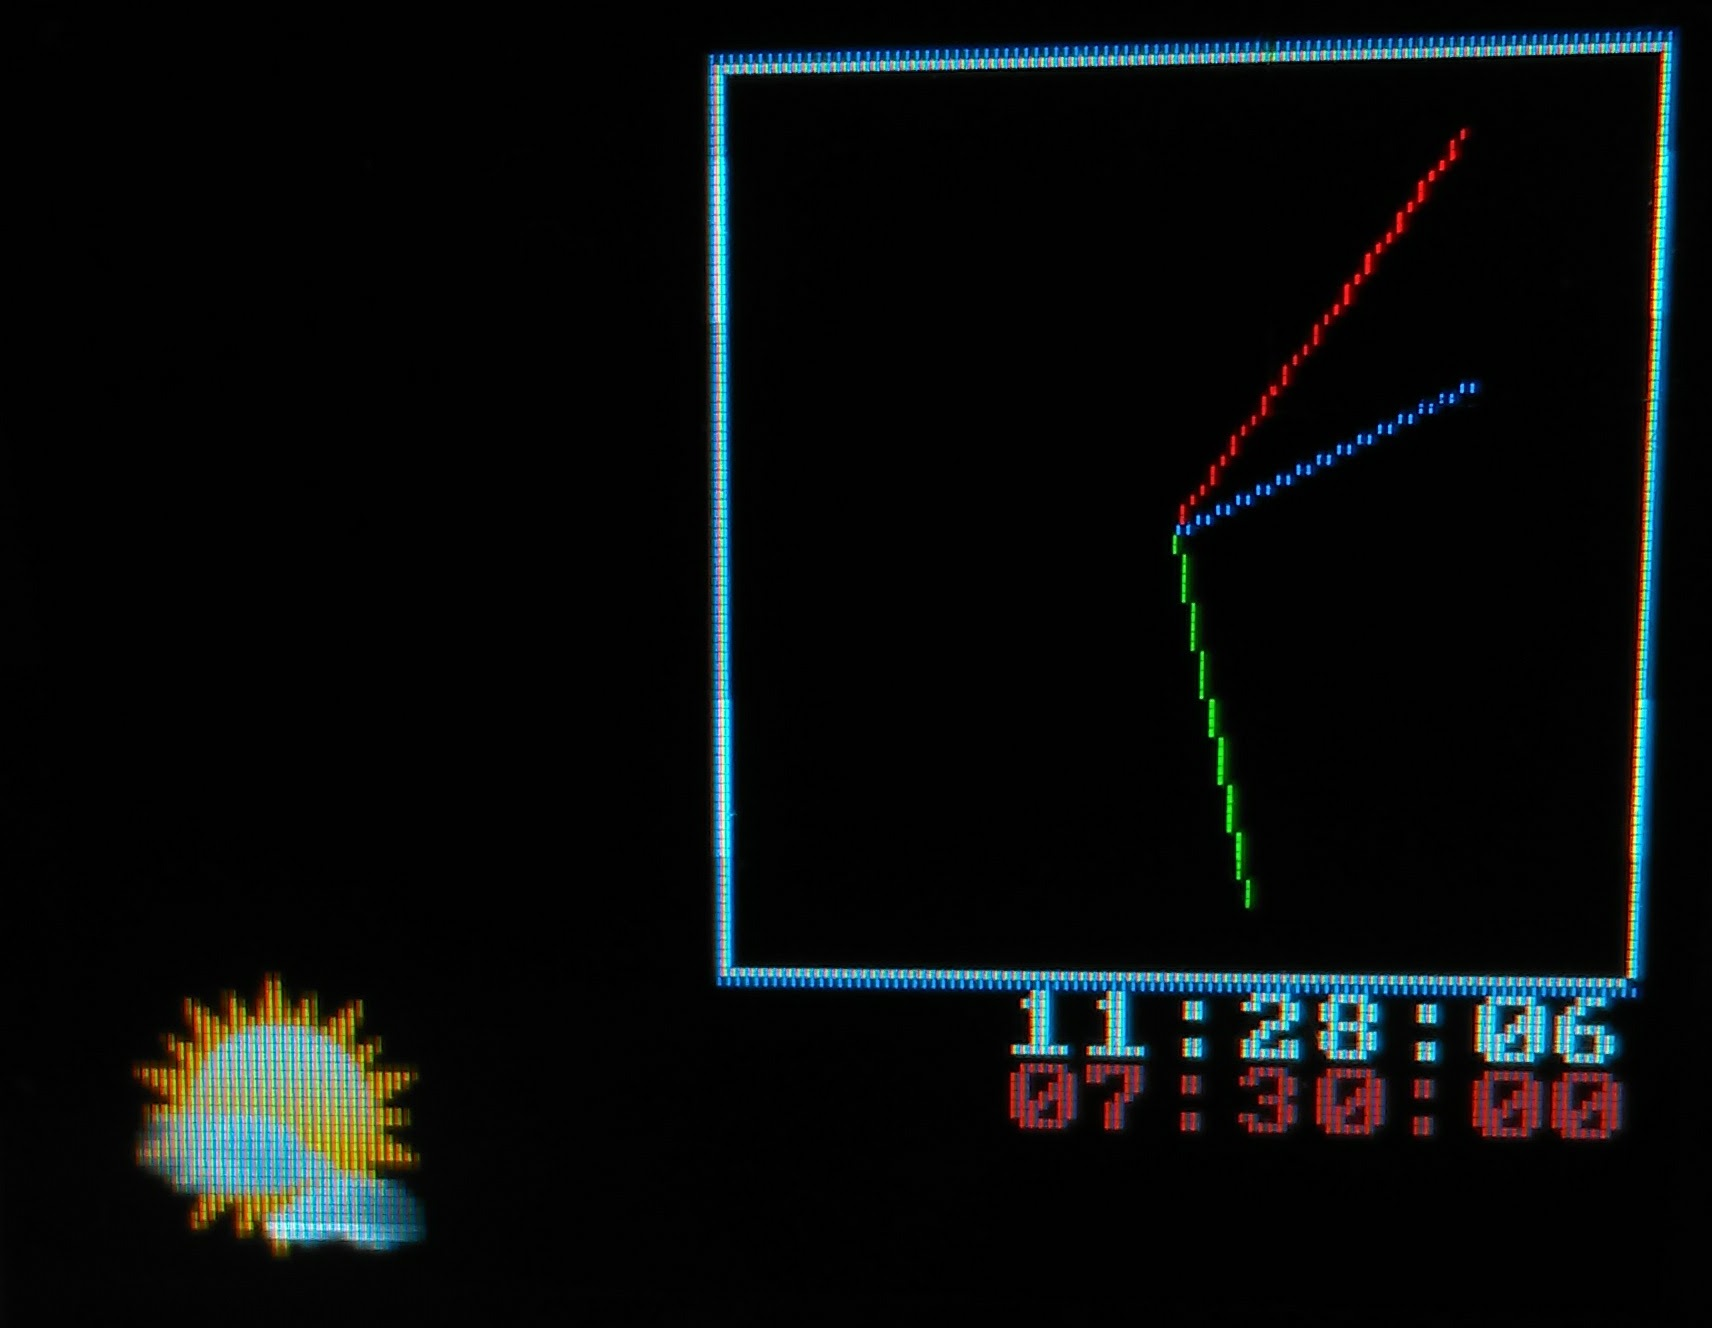
\includegraphics[width=0.4\textwidth]{./fig/clock_weather.png}
	\caption{Displaying the clock and the weather}
\end{figure}